\section{GEM based Readout}
\label{chap:TPC_sec:standard_gems}

Gas Electron Multipliers (GEMs) \cite{Sauli1997531} have been invented in the mid 90's. They consist of a thin polyamide foil, covered with Copper on both sides. Holes are produced into the foil on a regular pattern. Typical dimensions are a hole pitch of \SI{140}{\micro m} and a hole diameter of \SI{70}{\micro m}. If an electric field is applied between the two sides of the foil, high fields form inside the holes, and provide avalanche gas amplification. Since the high fields are constrained inside the holes, many of the high-voltage problems connected to traditional wire based chambers are not relevant. GEM foils can be stacked to provide tailored gas amplification. During the years a number of different types of GEM foils have been developed. They differ for example in the cross section of the holes, in the material of the foil, and in the pitch and hole sizes. For application in the ILC TPC currently two main options are being pursued. The first one is based on a GEM where a laser is used to ``drill'' each hole.
The resulting holes are
strictly cylindrical. The second option is based on a chemical etching process. The resulting holes have a double conical shape.

In addition to the different types of GEM foils two different schemes to build readout modules for the TPC are investigated. Scheme one (called module type A in the following) relies on a sturdy aluminum frame where the GEM foils are stretched between the bottom and the top of the readout module. This scheme allows to build a module which has essentially no dead area on the side of the module, but where some dead space is needed on the top and the bottom. The second option (called module type B in the following) relies on an assembly of a stiff but thin ceramic frame which when glued to the GEM provides a self-supporting stiff assembly. The width of the frame is around one millimeter, so that in this approach a small dead area is present all around the module. Both approaches allow the stacking of GEM foils, and both are compatible with the installation of a gating GEM on top.

\subsection{Module Type A, ``Asian Module''}
\label{chap:TPC_sec:asian_gems}
Most recent update: 2016-03-28\\
Contact person: Akira Sugiyama(email: sugiyama@cc.saga-u.ac.jp)\\

The Asian modules use GEM stacks as a gas amplification stage and are optimised to reduce the insensitive area
on the sides of the modules which point towards the detector center.
A module can be seen in figure \ref{fig_Fig1asiangempicture}.

\begin{figure}[!htb]
  \centering
  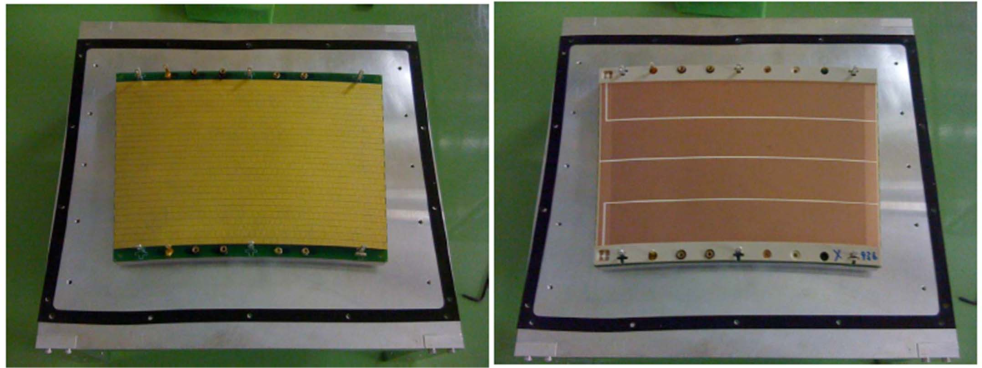
\includegraphics[width=0.9\textwidth]{Tracker/TPC_Bonn/plots/TPC-AG_Fig1asaingempicture}
  \caption{Asian GEM picture: left - anode pad plane; right - segmented cathode.}
  \label{fig_Fig1asiangempicture}
\end{figure}

Particles from the interaction point passing
between the modules may not be detected if they have very high momenta. Therefore, the Asian module foresees no frame along
the sides and extends the sensitive
area up to the edge of the backframe. To ensure a flat mounting of the GEMs, they are stretched on both the upper
and lower arcs (as seen in figure \ref{fig_Fig1asiangempicture}) which are made of a stiffer material:
GEMs with an insulator of \SI{100}{\micro\meter} Liquid Crystal Polymer (LCP)
covered with \SI{5}{\micro\meter} copper on both sides were produced by a company named SciEnergy.
The holes were
produced by \ce{CO2}-laser drilling after which they were carefully cleaned by dry etching to remove potentially
conductive residuals from the insides of the holes. The
hole pattern is identical to standard CERN GEMs. Because of the thicker material also higher gas gains per GEM
can be reached and a double GEM
structure is used and considered to be sufficient.
The two GEMs are mounted with an induction gap of \SI{2}{mm} and a transfer gap of \SI{3}{mm}.

The pad size is $1.2 \times \SI{5.4}{mm}$ and there are 28 pad rows with a total of 5152 pads.
From the beginning the use of an ion gate
(see subsection \ref{chap:TPC_sec:gating}) was envisaged and, thus, the level of the first GEM was designed
to be 1 cm below the nominal module height allowing for a later addition of the gate. To absorb the strength necessary
to stretch the GEMs and the gate, strong metal poles were implemented at the top and bottom arc.

\subsubsection{Recent Milestones}

All modules have been tested in the Large Prototype at DESY. The experience gained during all test beam periods as
well as the best transverse spatial resolution is described next. The testbeam measurements have used
the gas mixture of Ar-\ce{CF4}(3\%)-isobutane(2\%). The electric drift field was set in most cases to
E=\SI{230}{V/cm}, which is close to the maximum of the drift velocity, and alternatively to
E=\SI{130}{V/cm}, which is the minimum of the transverse diffusion.
The Asian modules were also measured using a laser system, in order to analyze the distortions.
The laser beam was scanned across the module, and the deviations were compared with calculations and are understood.

The Asian groups built three modules and made several test beam measurements at DESY (2009, 2010, 2012).
The first campaigns were dominated by very strong field distortions because of the mounting pins and the bare frames.
After introducing the field shaper, the distortions are comparable to the ones of other techniques used for modules.
The transverse spatial resolution is shown in figure \ref{fig_Fig2asiangemresolution}, where the measured spatial
resolution of a single row in the middle of a module can be seen.

\begin{figure}[!htb]
  \centering
  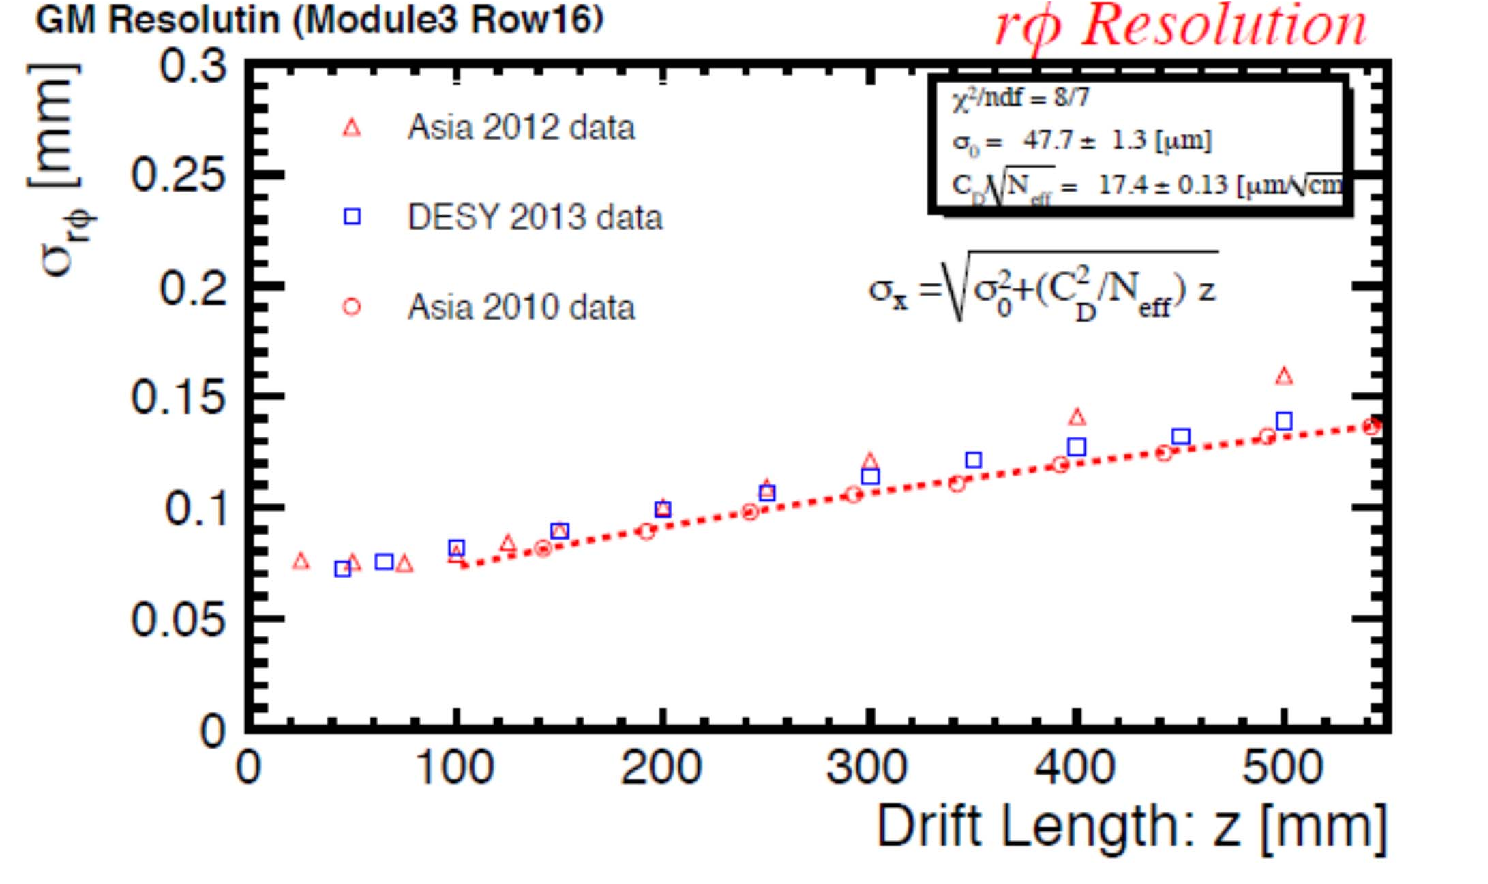
\includegraphics[width=0.9\textwidth]{Tracker/TPC_Bonn/plots/TPC-AG_Fig2asiangemresolution.pdf}
  \caption{Resolution measured for the Asian GEMs, and compared with a result for the DESY GEMs.}
  \label{fig_Fig2asiangemresolution}
\end{figure}

In this context an analytical formula was developed to predict the spatial resolution of a TPC. This formula includes
not only the effect of diffusion, angle,
noise and a finite pad-size, but also the influence of the electronics threshold, number of effective primary electrons,
the Polya-parameter of the gas
amplification, cross talk between pads and signal lines, charge loss because of attachment and the pad response function
are taken into account. All
these parameters can be varied and, if correctly chosen, describe well the measured data.

Finally, one other important observation was the HV micro-discharges on the Asian GEMs, with associated gain drops,
and investigations of this problem are summarized here.

To minimize the energy released in a discharge, the GEMs were segmented into four arcs, each with an area of
about $\SI{100}{cm^2}$ (figure \ref{fig_Fig1asiangempicture}, right).
Studies of the micro-discharges for the various types of GEMs were measured under a controlled environment.
The \SI{100}{\micro\meter} Asian GEMs discharged frequently, while the DESY \SI{50}{\micro\meter} GEMs (made by CERN) had little or no
discharges. For the \SI{50}{\micro\meter} GEMs, there is no significant difference of
the discharge rate between different types of GEMs. It is noteworthy that, at low gain, the \SI{100}{\micro\meter} GEMs
had a discharge rate which is almost the same as for the \SI{50}{\micro\meter} GEMs. The water content in the gas does not seem to
influence the
discharge rate, and long-term measurements are in progress.


\subsubsection{Future Plans}

In the future, it is planned to:\\
$\bullet$ understand better the reasons for the micro discharges and eliminate them, and \\
$\bullet$ construct a full scale Asian module with gate.

\subsection{Module type B, ``DESY Module''}
\label{chap:TPC_sec:DESY_gems}
Most recent update: 2016-03-28 \\
Contact person: Ties Behnke (email: ties.behnke@desy.de)\\

The goal of module type-B is a maximal coverage of the endplate with minimal dead area and a low material budget. It relies on thin ceramic frames to support the GEM foils on top of the readout plane \cite{Hallermann:2010zz,2012arXiv1202.6510D}, see figure \ref{fig:moduleAssembled}. The high stiffness of the ceramic frame allows the construction of very thin frames, which in turn minimize the dead areas of the module. With the current design only $\sim5\%$ of the active area is taken by the support structure and gaps between modules, the rest is sensitive area. The design of the system allows the simple stacking of GEM foils to build up compact, light weight self supporting multi-GEM modules. The development of this module type is led by DESY.

\begin{figure}[htb!]
\begin{subfigure}[b]{0.48\textwidth}
\includegraphics[width=\textwidth]{Tracker/TPC_Bonn/plots/TPC-DG_GemModule_Explosion.pdf}
\caption{}
\label{sfig:moduleExp}
\end{subfigure}
\hfill
\begin{subfigure}[b]{0.48\textwidth}
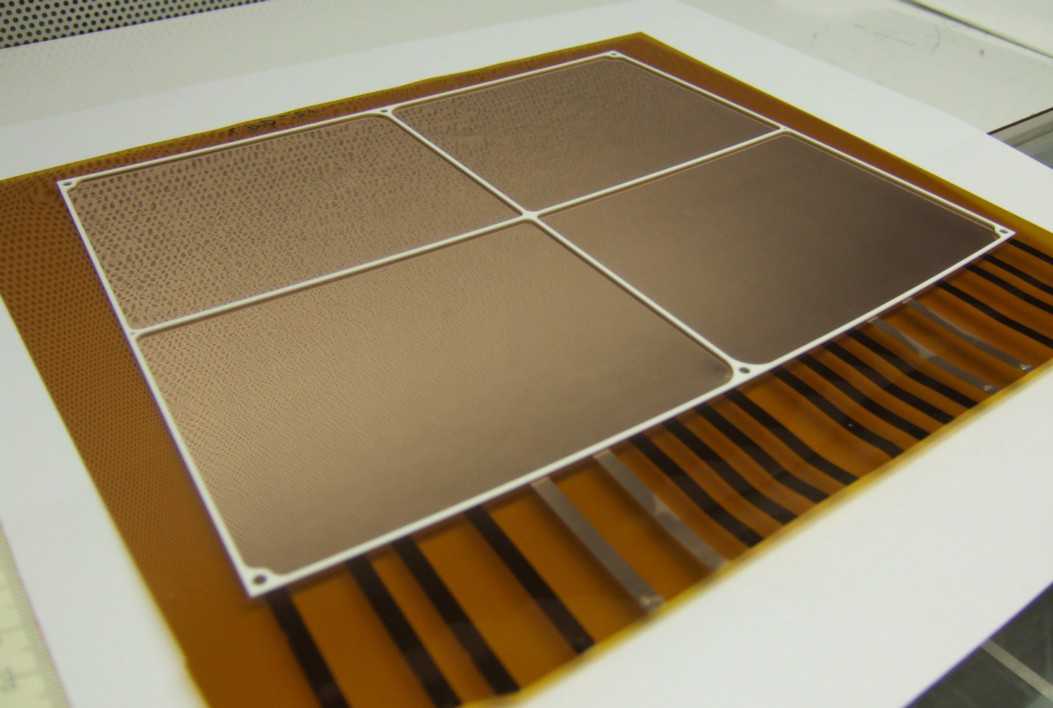
\includegraphics[width=\textwidth]{Tracker/TPC_Bonn/plots/TPC-DG_GemGrid.png}
\caption{}
\label{sfig:moduleGEM}
\end{subfigure}
\caption [Readout Module GEM]{\small \protect\subref{sfig:moduleExp})~Exploded view of one module showing the sequence of GEM foils and ceramic frames. \protect\subref{sfig:moduleGEM})~GEM foil with ceramic frame support used in the construction of the modules.}
\label{fig:moduleAssembled}
\end{figure}

\subsubsection{Recent Milestones}
Over the last years several test-beam campaigns took place and exposed three GEM based modules to test beam. Extensive data sets were collected with and without magnetic field, at different working points, and at different angles between the TPC and the beam.

For the first time the data taken were used in a global attempt to determine and correct field distortions. The Millepede-II \cite{Blobel20065,millepedeWiki} program was used to perform this global fit. First results indicate that distortions as large as several millimeters can be well corrected, see figure \ref{sfig:1Tdistort}. The resolution obtained both in $r\text{-}\varphi$ and $z$ behave as expected, and, if extrapolated to the running conditions at the ILC, meet the requirements, see figure \ref{sfig:resextrapol}.

\begin{figure}[htb!]
\begin{subfigure}[b]{0.48\textwidth}
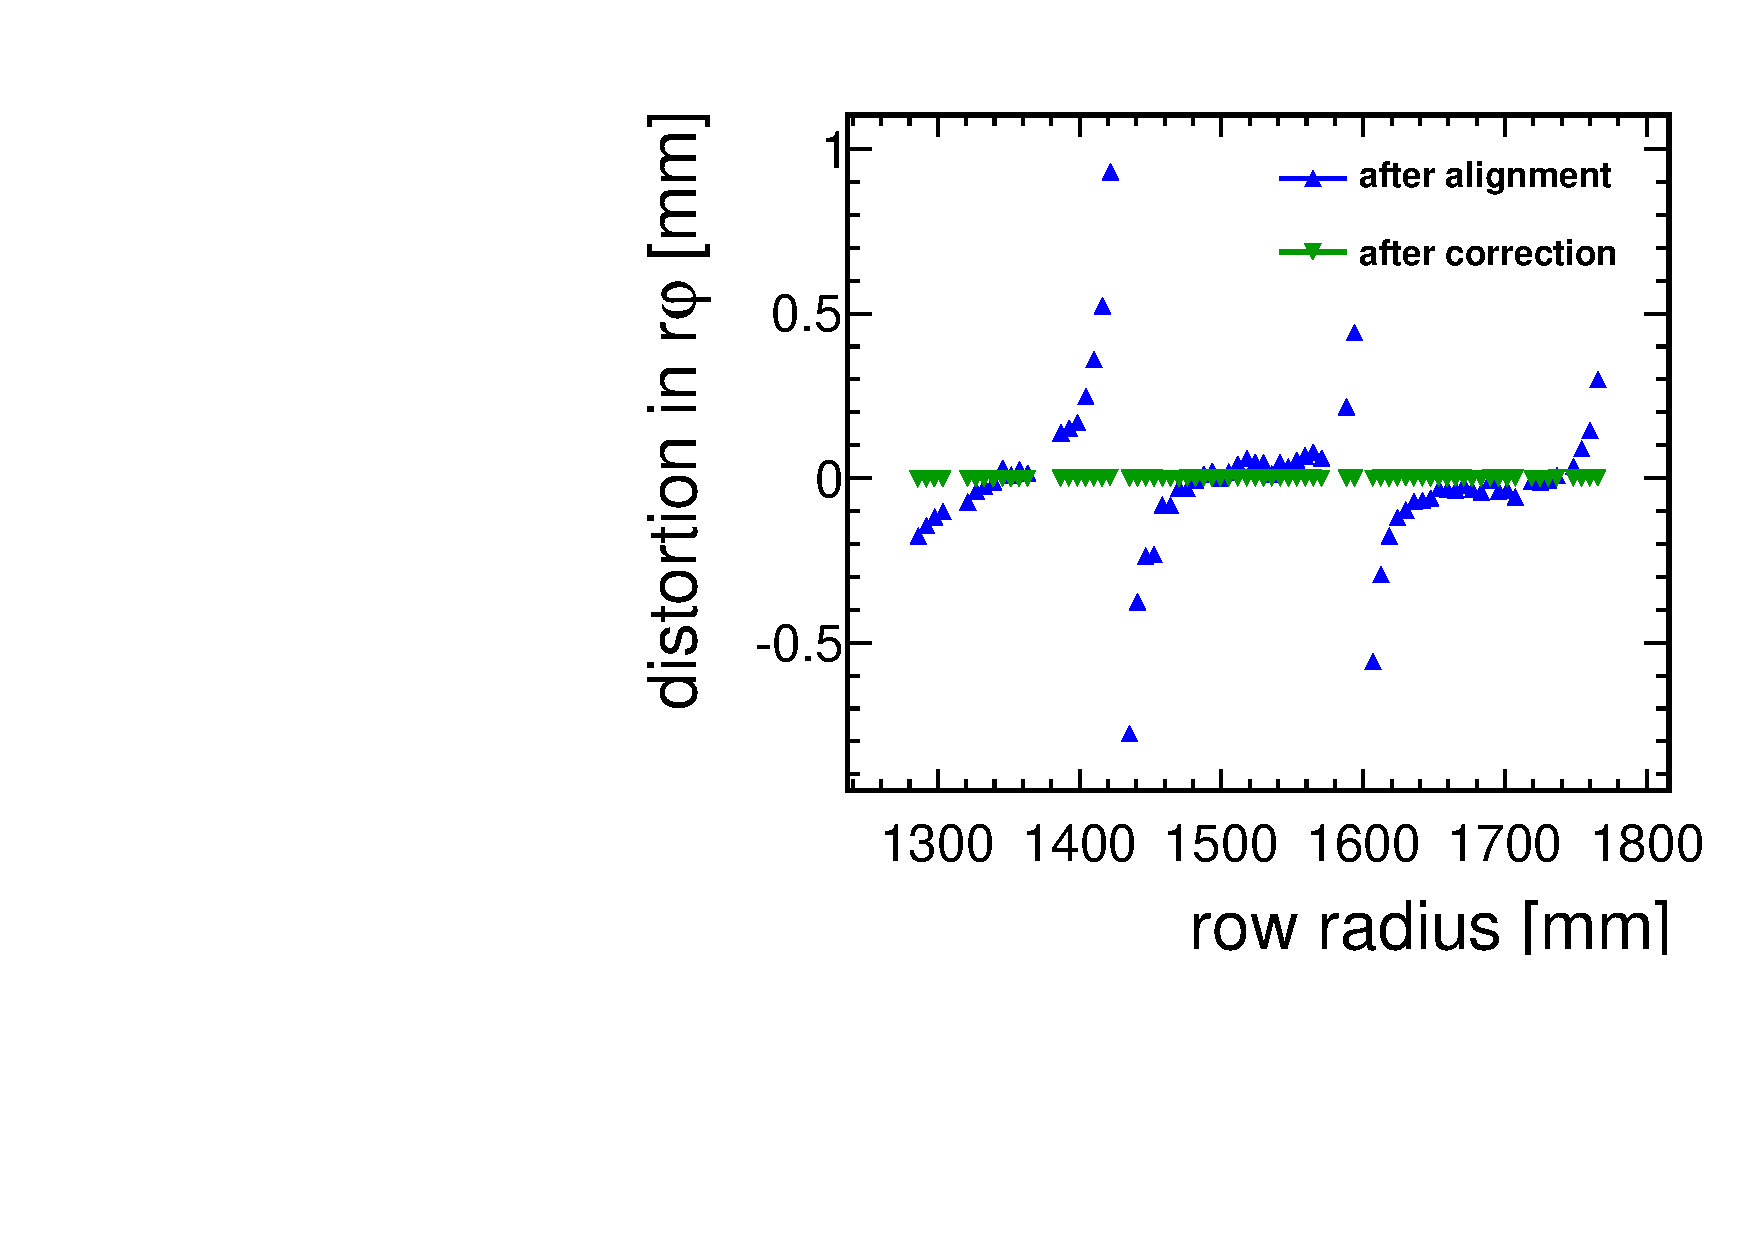
\includegraphics[width=\textwidth]{Tracker/TPC_Bonn/plots/TPC-DG_distortionAlignmentPaper1Tdistcor.pdf}
\caption{}
\label{sfig:1Tdistort}
\end{subfigure}
\begin{subfigure}[b]{0.48\textwidth}
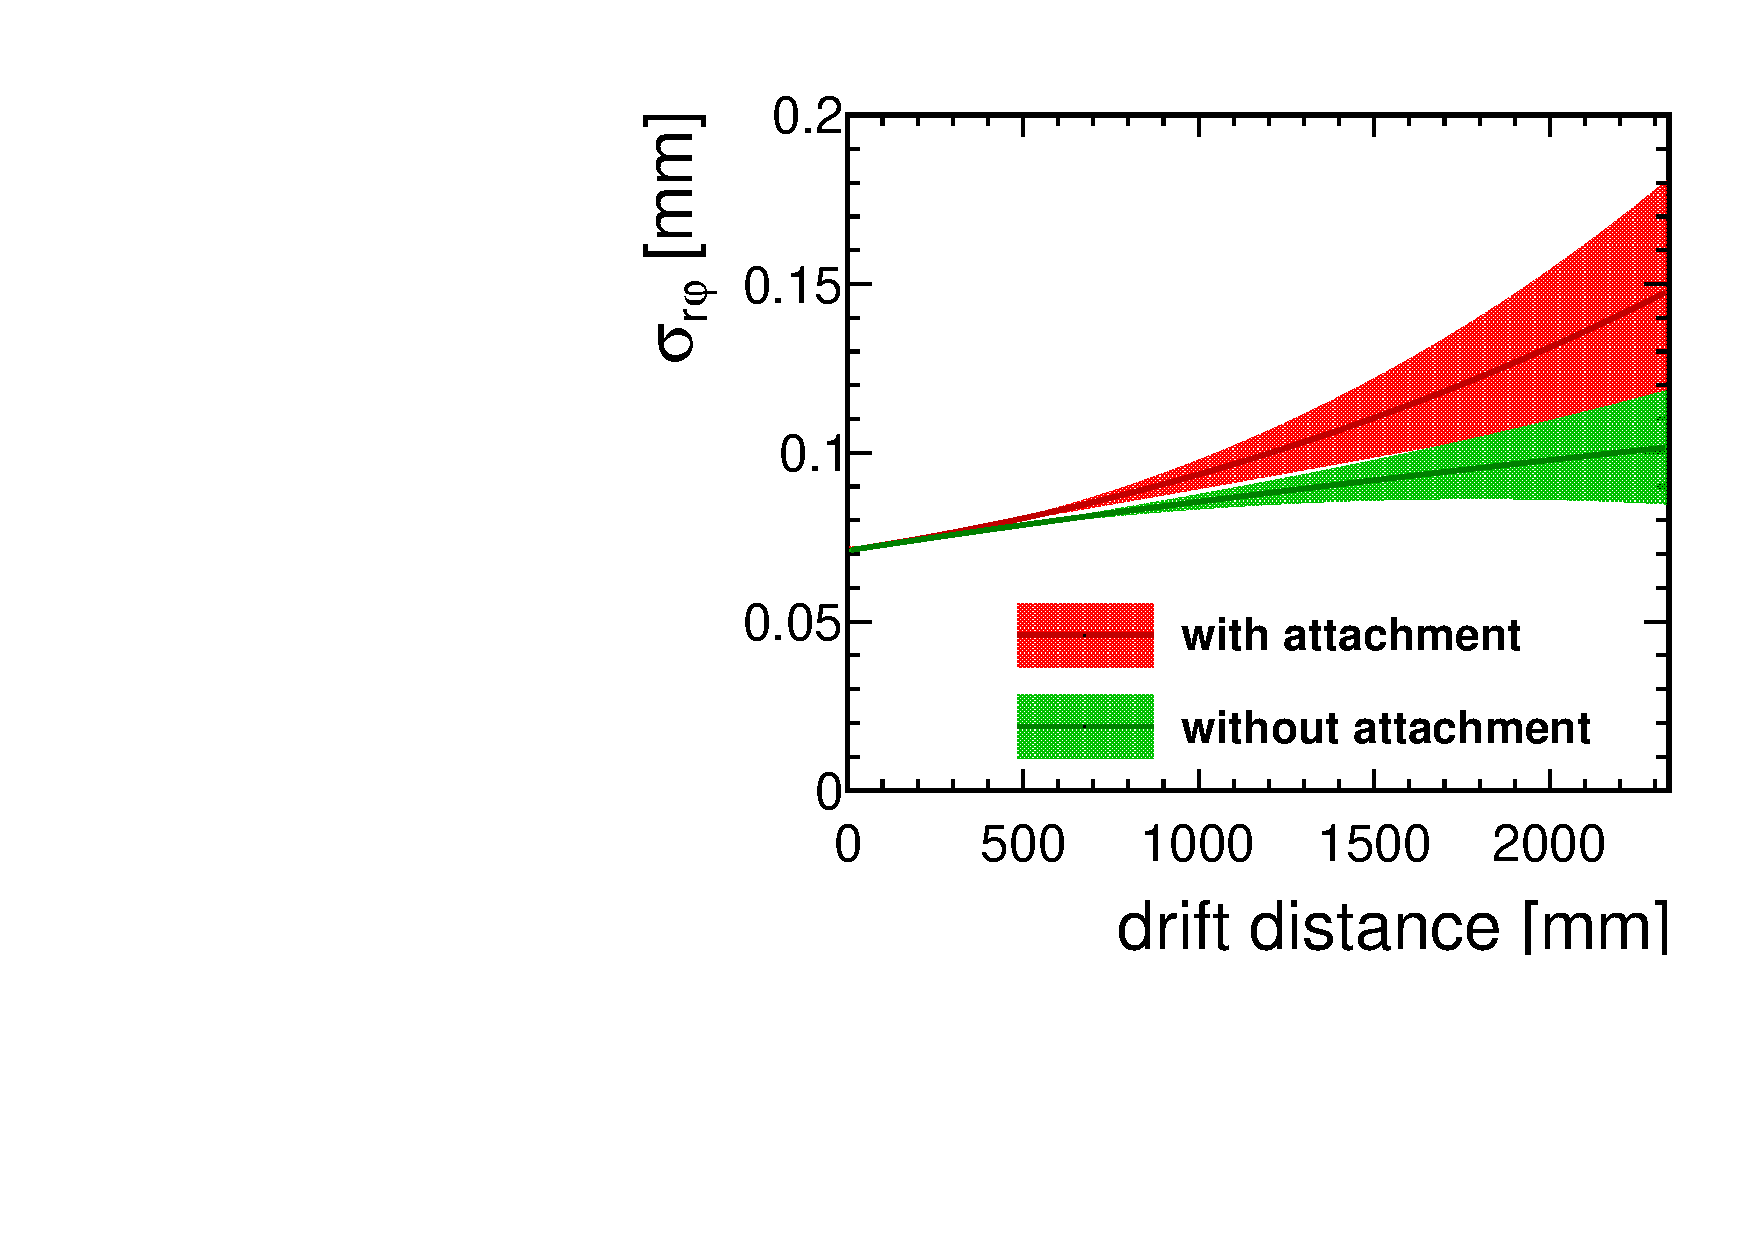
\includegraphics[width=\textwidth]{Tracker/TPC_Bonn/plots/TPC-DG_xyResolutionExtrapolated.pdf}
\caption{}
\label{sfig:resextrapol}
\end{subfigure}
\caption{\small \protect\subref{sfig:1Tdistort})~Alignment and distortion correction: mean hit position in $r\varphi$ with respect to the track position at \SI{1}{T} versus pad row radius. In blue after alignment correction, in green after distortion correction. \protect\subref{sfig:resextrapol})~Point resolution: extrapolation to a magnetic field of \SI{3.5}{T} based on parameters measured with the Large TPC Prototype at \SI{1.0}{T}. Plotted over the full ILD TPC drift length of \SI{2.35}{m} including 1 \sigma error bands. In red with the measured attachment rate, in green without any attachment.}
\label{fig:align1Tdistort}
\end{figure}

The field homogeneity was in addition studied in dedicated laser runs \cite{Zenker:2014qra}. A UV laser illuminates the cathode plane in the TPC, on which dots are placed made from a material with a small work function. The laser light extracts electrons at the position of the dots. These electrons are then drifted towards the anode, and are measured. From the dislocations of the dots relative to the known position on the cathode, the integrated effect of field distortions in the TPC volume can be measured.

Extensive simulations of the behavior of the GEM foils in case of electrical breakdown were performed. They showed that a strong coupling exists between the different regions of the GEM foil. In some cases these couplings can trigger secondary trips in the module, which in rare cases can damage the GEM. A protection circuit is currently under development and will be tested in the near future.

%\subsubsection{Engineering Challenges}
\subsubsection{Future Plans}

By now two generations of these modules have been developed and successfully tested. The main issues which are going to be addressed in the next 1-2 years are
\begin{itemize}
\item re-optimisation of the support structure for maximum mechanical strength and minimal interference with the readout
\item development of a protection scheme which will ensure safe operation of the module even in case of high-voltage trips.
\item optimization of the field-shaping integrated into the module, to minimize field distortions close to the module and at module boundaries.
\item integration of a GEM based gate on top of the current amplification structure, based on the recent developments at KEK.
\end{itemize}
It is planned that within the next six months a third generation module design will be developed and several modules built which will address these challenges.

\subsubsection{Engineering Challenges}
%The GEM based modules face rather similar engineering challenges. Among the most important one is the optimisation of the overall mechanical structure, to provide adequate mechanical strength, without introducing excess dead material.
A detailed study is ongoing to understand and quantify the mechanical behavior of the ceramic frame GEM system. Bending tests have been performed, and compared to simulations. The interference between the mechanical properties and the electrical properties are studied. Measurements of the flatness of the module are being done, and will provide input for the next design iteration.
The fabrication of the ceramic frames which is currently done by laser cutting from solid sheets of ceramic will be studied. Possible alternatives are 3D printing of the frames. Improvements in the laser cutting technology might allow thinner frames, without loosing stiffness.

Another open question is the distribution of the high voltage from the endplate to the different GEM layers. The current solution is rather labour intensive, and relies heavily on the skills of the person doing this connection. Faults are difficult to find, and even more difficult to repair. Here new solutions are being sought, which are more easily to produce, more reliable, and will give better high voltage security. Connected to this are the protection schemes against accidental high voltage discharges, which are still not perfect.

As discussed in section \ref{chap:TPC_sec:gating}, a gating GEM will be implemented as part of the amplification scheme. This gating GEM needs to be mechanically integrated into the module.

Currently a gap of about \SI{2}{mm} exists between neighboring modules. This gap introduces significant field distortions \cite{Zenker:2014qra}. They are partially compensated by a field shaping strip on the outside of each module. However a better and more robust solution would be to further minimize the gap between modules. Doing so will need improvements of the high voltage distribution, as discussed above, but also of the overall mechanical integration of the modules into the endplate.

%\subsection{Applications Outside of Linear Colliders}

